\documentclass{article}
\usepackage[utf8x]{inputenc}
\usepackage{lipsum}
\usepackage[margin=1in,includefoot]{geometry}
\usepackage{fancyhdr}
\pagestyle{fancy}
\usepackage{graphicx}
\usepackage{amssymb}
\usepackage{pifont}
\newcommand{\cmark}{\ding{51}}
\newcommand{\xmark}{\ding{55}}
\usepackage{listings}
\usepackage{color}
\usepackage{hyperref}
\usepackage[table]{xcolor}
\usepackage{float}
\usepackage{longtable}
\usepackage[T1]{fontenc}
\usepackage{textcomp}
\usepackage[english]{babel}
\usepackage[T1]{fontenc}
\usepackage{uarial}
\renewcommand{\familydefault}{\sfdefault}
\definecolor{dkgreen}{rgb}{0,0.6,0}
\definecolor{gray}{rgb}{0.5,0.5,0.5}
\definecolor{mauve}{rgb}{0.58,0,0.82}
\hypersetup{
    colorlinks=true, % make the links colored
    linkcolor=black, % color TOC links in blue
    urlcolor=blue, % color URLs in red
    linktoc=all % 'all' will create links for everything in the TOC
}
\lstset{
    commentstyle = \color{gray},
    extendedchars = \true,
    inputencoding = utf8x,
    language = php,
    keepspaces = true,
    keywordstyle = \bfseries,
    backgroundcolor = \color{blue!25},
    xleftmargin = 2cm,
    framexleftmargin = 1em
}
\colorlet{punct}{red!60!black}
\definecolor{background}{HTML}{EEEEEE}
\definecolor{delim}{RGB}{20,105,176}
\colorlet{numb}{magenta!60!black}
\lstdefinelanguage{json}{
    basicstyle=\normalfont\ttfamily,
    numbers=left,
    numberstyle=\scriptsize,
    stepnumber=1,
    numbersep=8pt,
    showstringspaces=false,
    breaklines=true,
    frame=lines,
    backgroundcolor=\color{background},
    literate=
     *{0}{{{\color{numb}0}}}{1}
      {1}{{{\color{numb}1}}}{1}
      {2}{{{\color{numb}2}}}{1}
      {3}{{{\color{numb}3}}}{1}
      {4}{{{\color{numb}4}}}{1}
      {5}{{{\color{numb}5}}}{1}
      {6}{{{\color{numb}6}}}{1}
      {7}{{{\color{numb}7}}}{1}
      {8}{{{\color{numb}8}}}{1}
      {9}{{{\color{numb}9}}}{1}
      {:}{{{\color{punct}{:}}}}{1}
      {,}{{{\color{punct}{,}}}}{1}
      {\{}{{{\color{delim}{\{}}}}{1}
      {\}}{{{\color{delim}{\}}}}}{1}
      {[}{{{\color{delim}{[}}}}{1}
      {]}{{{\color{delim}{]}}}}{1},
}

\begin{document}
\rowcolors{2}{teal!20}{white}
\begin{titlepage}
\begin{center}
\begin{figure}[H]
\centering
\end{figure}
\line(1,0){350}\\
\huge{\bfseries Zaakpay Integration Document}
\line(1,0){250}\\
[1.5cm]
\textsc{\Large Version 2.0}
\end{center}


\end{titlepage}
\thispagestyle{empty}
\tableofcontents
\thispagestyle{empty}
\newpage
\listoffigures
\listoftables
\thispagestyle{empty}
\cleardoublepage
\setcounter{page}{1}
\section{Introduction}\label{sec:Intro}
Zaakpay is an online payments platform that offers multiple payment methods to both an individual user and a business. 

So, whether you are an ecommerce giant, a small spunky start-up or an individual user simply wanting to make payments to businesses, we have products that cater to all your needs.

This document describes the steps for technical integration process between merchant website/app and Zaakpay Payment Gateway for enabling online transactions. This document is covered in two sections. Section 1 covers website integration and Section 2 covers the APIs provided to the merchants.

\section{Sign-Up}
Signup for a business account on Zaakpay. After signing up and verifying your account
follow the steps below:
\begin{itemize}
\item  Login to Zaakpay on \url{https://www.zaakpay.com}
\begin{figure}[H]
\centering
\caption{Sign-Up}
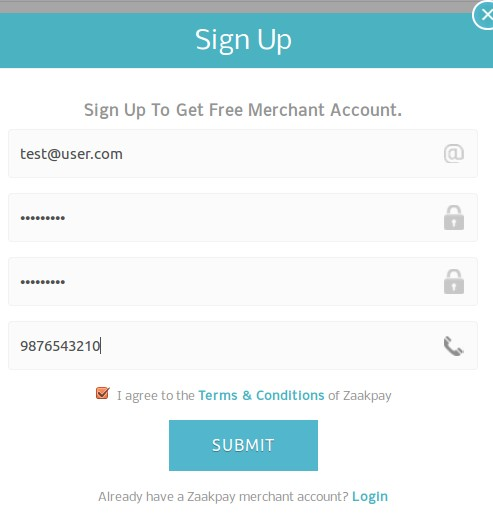
\includegraphics[width=0.8\textwidth,height=4.3in]{Signup1.png}
\end{figure}
\item  Click the My Account tab.
\item  Select the integration sub-menu item under the My Account tab.
\item   Select the URLs \& Keys tab from the navigation.
\item  Fill in details like the domain you'll be posting from and your return URL.Here the domain is the domain where you'll be posting data to Zaakpay from and the response URL for transact API is the path to the response.ext file on your server.
\item Select the Transaction limits sub-menu item under the My Account tab and set your appropriate transaction limits.
\end{itemize}
 \begin{figure}[H]
\centering
\caption{Dashboard-Home}
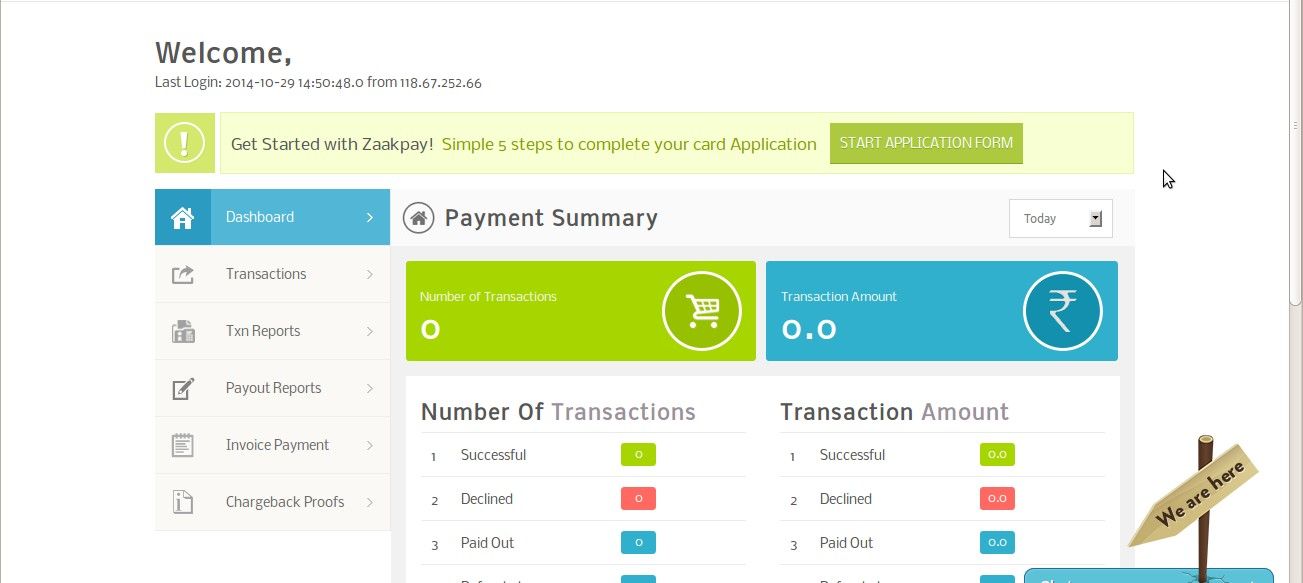
\includegraphics[width=1.1\textwidth,height=4.2in]{Zaakpay_panel.png}
\end{figure}
Generate your secret key and note it down along with your merchant identification
number.

\newpage
\section{Get Merchant ID and Secret Key}
Login to your Zaakpay account with registered email id. Go to Integration section. You’ll get your Merchant Identifier and Secret key in URLs and Keys section. \\
\begin{figure}[H]
\centering
\caption{Dashboard-Developer Section}
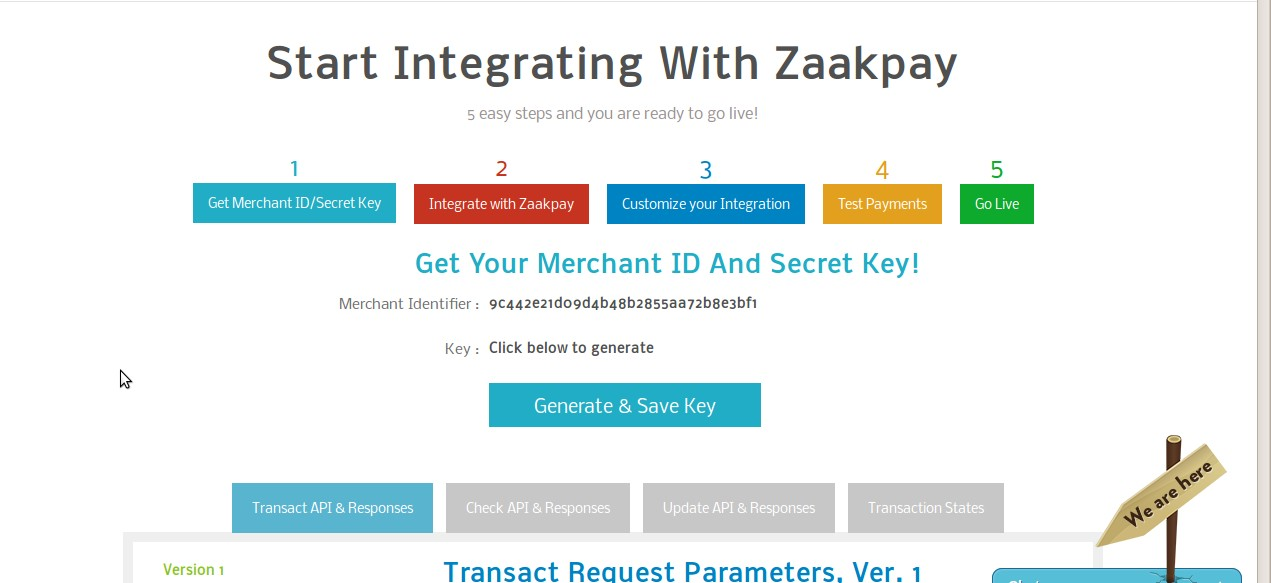
\includegraphics[width=1\textwidth,height=3.3in]{Zaakpay_panel1.png}
\end{figure}

If Secret key is blank, you can generate Key by pressing the button “Generate Key” and save. If you're using the integration kit, please replace the values of the secret key in the response.ext and posttozaakpay.ext files where ext=extension.

Next, you need to fill in the domain details in your Zaakpay account. For that, click on "Customize your Integration" and then, click on "URL's" as described in the screen below.

\begin{figure}[H]
\centering
\caption{Dashboard-URL section}
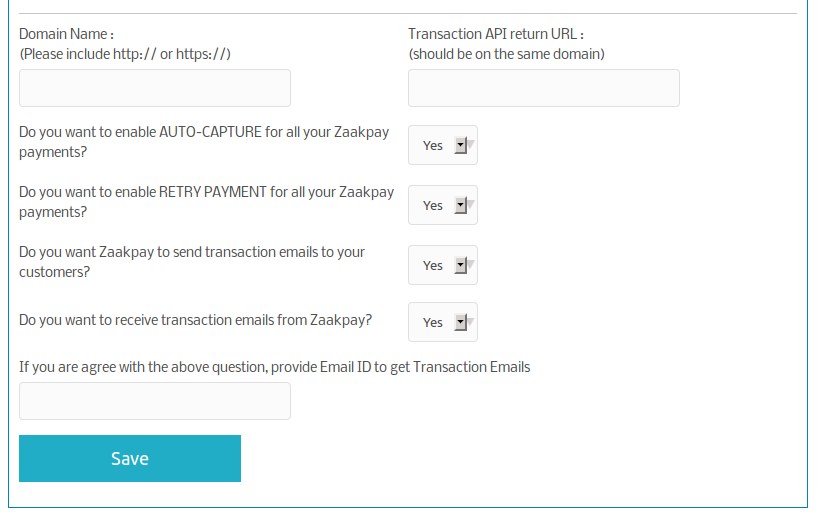
\includegraphics[width=0.8\textwidth,height=3.1in]{Data_not_complete.png}
\end{figure}

After this, proceed to the next tab, "Transaction Limits". Here you can update the transaction caps (upper and lower) as per your requirements.

\begin{figure}[H]
\centering
\caption{Dashboard-Transaction Limits}
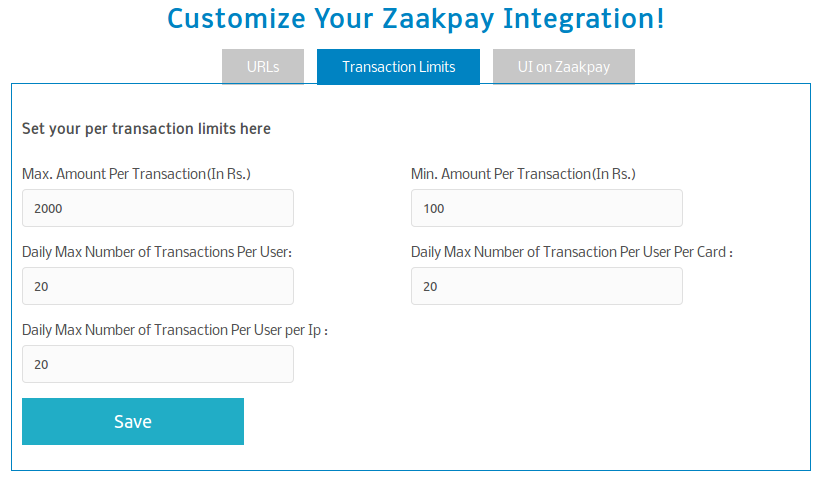
\includegraphics[width=0.8\textwidth,height=3.3in]{Transaction_limits.png}
\end{figure}

Next you can complete the integration UI by uploading a brand image on the ext tab.

\begin{figure}[H]
\centering
\caption{Dashboard-UI section}
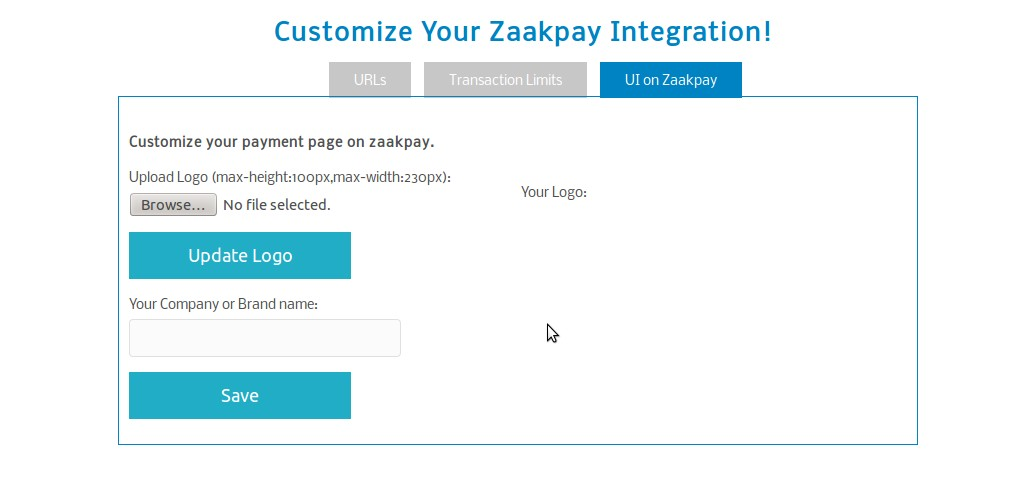
\includegraphics[width=0.8\textwidth,height=3.3in]{Zaakpay_ui.png}
\end{figure}
Click on "Save" once you are done with all these configurations.
\\

This was the overall set of procedures required for Zaakpay integration at our end. Next comes Merchant's side of integration, which is explained in the later sections.


\newpage
\section{Staging Credentials}
\begin{itemize}
\item {\bfseries URL : } http://zaakpay-staging.cloudapp.net:8080
\item {\bfseries Merchant Identifier :} b19e8f103bce406cbd3476431b6b7973
\item {\bfseries Secret key :} 0678056d96914a8583fb518caf42828a
\item {\bfseries Public KeyId :}
sAMtcgidueVcrZI
\item {\bfseries Public key :} MIIBIjANBgkqhkiG9w0BAQEFAAOCAQ8AMIIBCgKCAQEAikG2PaW+CqT3m\\26Dbtm7una22MYEDd+xONYjwE69Qa/FNQO0R5eqUnfi4lneWX6rc1IB6iVhyNDYULOZB\\W7vUsFbDWNJFDTD+V1T+30VXYvo+m7ufZCgxJVLn8W+JnKn1JPaL0n78UV2cG9zPlXK\\zJcMIGrNSG9QWFd6XJjlriJ2CFEbzPf7a4y7DwNgGrRpqMkmJDHNLcaba+CtTqjgeGUWo\\VIIg7RaQk4rJ5v21qyVK0pAUyfEXBDcLGWjsae0lsK+En7RFpV5NV6HxO78RnfT07RIdIBH\\xjWeM9WJ+xuGBKrODXmKRdWXSCAIiDYCp6F6fkgViE1XnCL6gQbnqQIDAQAB
\end{itemize}
\newpage
\section {Checksum Calculation}
For both integrity \& data-authenticity verification before sending data to the API, you need to calculate a checksum of all the data that you send to Zaakpay. We use an HMACSHA- 256algorithm to calculate the checksum of ALL data that is posted to the API. We require data to be posted to our server in NVP (Name-Value Pairs) format.
\\ To calculate the checksum please follow the process below:
\begin{itemize}
\item Calculate the checksum using the HMAC SHA-256 algorithm using the string as data parameter and your generated secret key.
\item The resulting checksum calculated should be posted to the Zaakpay API along with other data. For example: Let's suppose we need to post the following data to the API. We calculate "checksum" only with the parameters mentioned below and the order of the parameters must remain intact when calculating "checksum".
\end{itemize}

For more on HMAC implementations for various platforms please take a look at the following links:
 \begin{itemize}
\item \href{http://www.jokecamp.com/blog/examples-of-creating-base64-hashes-using-hmac-sha256-in-different-languages/#php}{PHP HMAC implementation}
\item \href{http://www.jokecamp.com/blog/examples-of-creating-base64-hashes-using-hmac-sha256-in-different-languages/#python}{Python HMAC implementation}
\item \href{http://www.jokecamp.com/blog/examples-of-creating-base64-hashes-using-hmac-sha256-in-different-languages/#perl}{Perl HMAC implementation}
\item \href{http://www.jokecamp.com/blog/examples-of-creating-base64-hashes-using-hmac-sha256-in-different-languages/#ruby3}{Ruby HMAC implementation}
\item \href{https://gist.github.com/tsupo/112188/acdbf002acf454bd60c355a776b9a5b58b6dff5e}{C HMAC implementation}
\item \href{http://www.jokecamp.com/blog/examples-of-creating-base64-hashes-using-hmac-sha256-in-different-languages/#java}{Java implementation}
\item \href{http://www.jokecamp.com/blog/examples-of-creating-base64-hashes-using-hmac-sha256-in-different-languages/#js}{JavaScript HMAC implementation}
\item \href{http://www.jokecamp.com/blog/examples-of-creating-base64-hashes-using-hmac-sha256-in-different-languages/#csharp}{.NET's System.Security.Cryptography.HMAC}
 \end{itemize}
The links provided above are for referential purposes only. The final checksum should be
converted into HEXADECIMAL character set.
\newpage
\section{Card Encryption}
\begin{itemize}
\item The public key (Present in your Zaakpay Profile) is stored, and used to encrypt the card details using RSA algorithm
\item You can find the public key on the path : 
\begin{figure}[H]
\centering
\caption{Dashboard-PG keys}
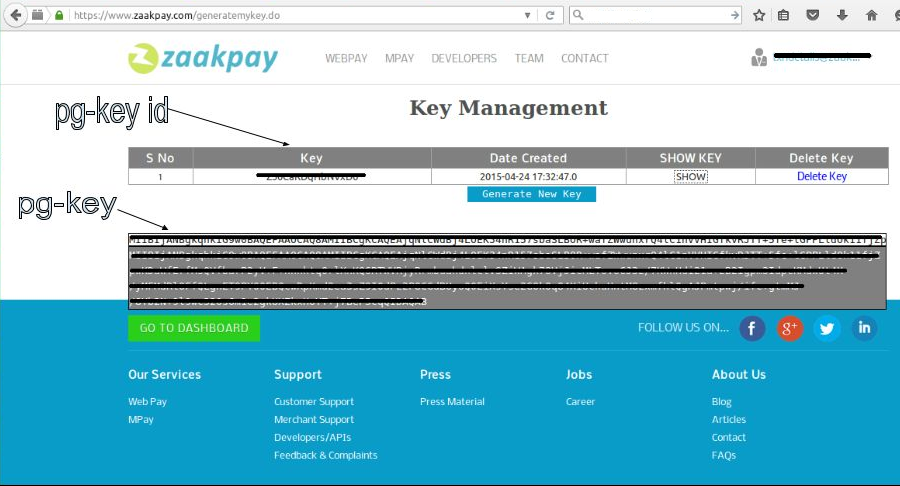
\includegraphics[width=1.15\textwidth,height=4.7in]{key.png}
\end{figure}
\newpage
\item The sample java code explains the flow
\begin{lstlisting}[language=java,breaklines=true]
public static String encrypt(String text) {
		byte[] cipherText = null;
		try {

			BASE64Decoder base64Decoder = new BASE64Decoder();

			byte[] decodedString = base64Decoder.decodeBuffer("your_pg_key");

			PublicKey publicKey = KeyFactory.getInstance("RSA").generatePublic(new X509EncodedKeySpec(decodedString));
			
			final Cipher cipher = Cipher.getInstance("RSA");
			
			cipher.init(Cipher.ENCRYPT_MODE, publicKey);
			String data= byteToBase64(cipher.doFinal(text.getBytes("UTF-8")));
			return data;
		} catch (Exception e) {
			e.printStackTrace();
		}
		return null;
		
	}

\end{lstlisting}
\item The card number, cvv, and expiry need to be encrypted using the same format before sending to Zaakpay
\item RSA encryption is used with PKCS1 Padding RSAES-PKCS1-v1\_5
\end{itemize}

\newpage
\section{Get Up Enabled Payment Options API}
This api will return the payment methods available to merchant (based on merchant id) and cards saved by a 
user. 

\begin{itemize}
\item Request Type:	GET 
\item Request URL (Staging): \url{http://zaakpay-staging.cloudapp.net:8080/getPaymentMethods}
\item Request URL (Live): \url{https://api.zaakpay.com/getPaymentMethods}  
\end{itemize}

\subsection{Request Parameters}


\begin{lstlisting}[language=json,breaklines=true]
data={ 
    "merchantIdentifier": "zaakpaymid", 
    "email":"abc@gmail.com", 
    "mode":"0" 
     } 
 &checksum=dfsafdsfdsf89345nvetvw4985vnery

\end{lstlisting}
\subsection{Response Parameters}
\begin{lstlisting}[language=json,breaklines=true]
{ 
    "email": "chirag@zaakpay.com", 
    "responseCode": "100", 
    "responseDescription": "Cards have been fetched successfully.", 
    "enabledNetbanking": { 
        "SBI": "State Bank of India", 
        "AXIS": "Axis Bank", 
        "KMB": "Kotak Mahindra Bank" 
    }, 
    "enabledCards": [ 
        "Visa", 
        "Master", 
        "Maestro", 
        "Diners", 
        "Discover" 
    ], 
    "cards": [ 
        { 
            "nameoncard": "chirag jain", 
            "first4": "4012", 
            "last4": "1881", 
            "cardId": "bce8e4e1e66520cb0bc2bf3a0e760412d53273a844bf0931f2b3136a2ee0ada3~1", 
      		"cardScheme": "Visa", 
            "cardToken": "4012 XXXX XXXX 1881", 
 "merchantCardRefId": "cardRef123" 
        }, 
        { 
            "nameoncard": "chirag jain",  
            "first4": "5610", 
            "last4": "8250", 
            "cardId": "dbd45ca21bedf7a7fb4156533e779e8aee5e7a89c46ba203c85c89f91bd21dd9~12", 
            "cardScheme": "Maestro", 
            "cardToken": "5610 XXXX XXXX 8250", 
 			"merchantCardRefId": "cardRef123" 
        } 
    ] 
} 
\end{lstlisting}


\newpage
\section{Transact API:Server-to-Server}
Using this api, merchant’s server POSTs card/bank data to Zaakpay’s server. Zaakpay’s server responds back 
with bank’s url.

\begin{itemize}
\item Request Type:	POST 
\item Request URL (Staging): \url{http://zaakpay-staging.cloudapp.net:8080/transactU?v=4}
\item Request URL (Live):	\url{https://api.zaakpay.com/transactU?v=4}
\end{itemize}

The flow of this integration is explained in the figure below :
\begin{figure}[H]
\centering
\caption{Integration Flow}
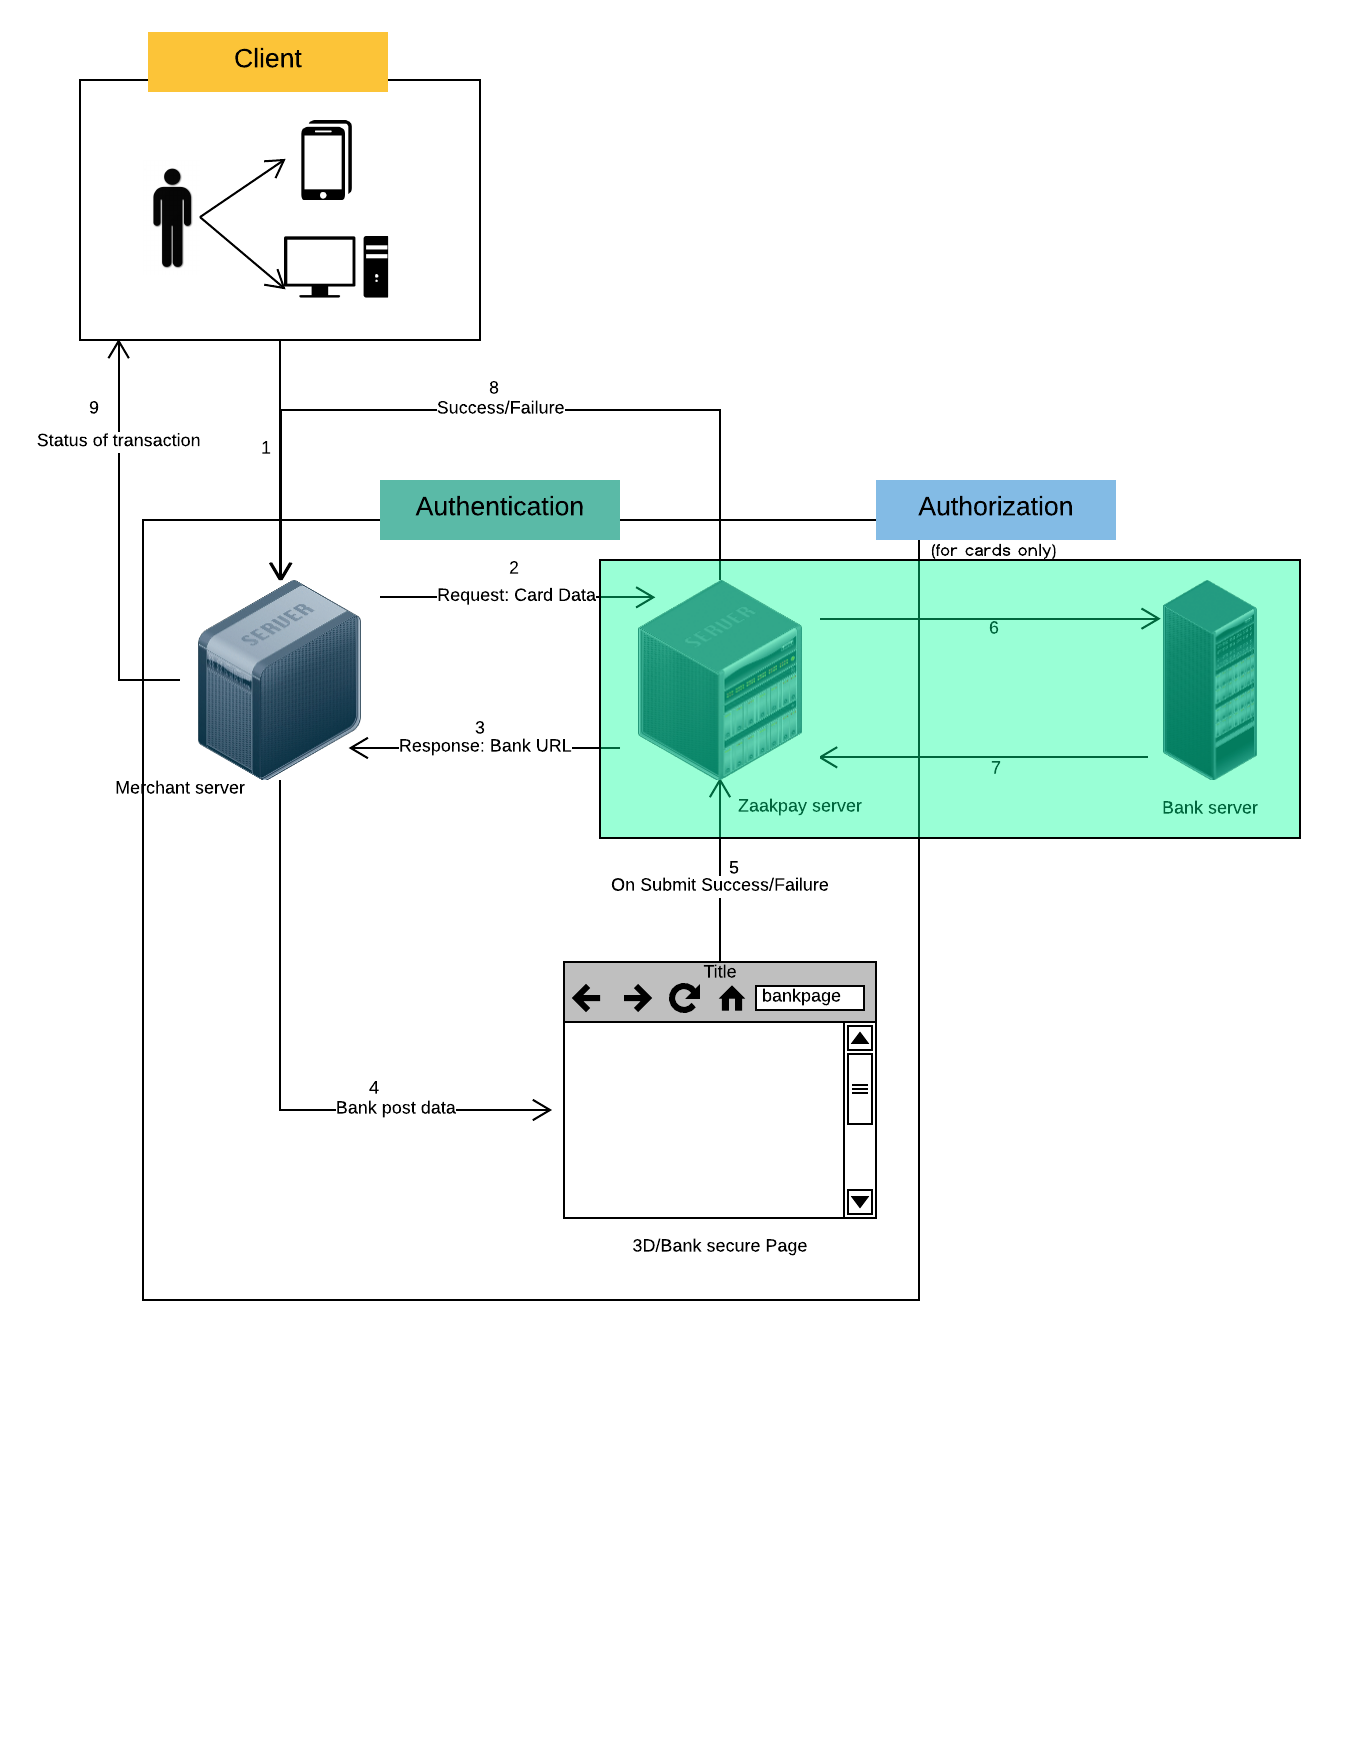
\includegraphics[width=1.2\textwidth,height=6.3in]{TransactU-_Flow.png}
\end{figure}


\subsection{Request Parameters}
\begin{longtable}{||c|| p{2.09cm}|| p{5.5cm}| p{4.7cm}||}
\caption{Transact API request}\\
\rowcolor{green!50}
\bfseries{Parameter} & \bfseries{Optional O, Mandatory M} & \bfseries{Validation} & \bfseries{Allowed Values} \\ \hline
merchantIdentifier & M & alphanumeric & Zaakpay's unique identifier for your website \\
orderId & M & max 20 alphanumeric,must be unique per website, we do not accept duplicate & Your unique transaction identifier. \\
returnUrl & O & This must be the domain(or a sub-domain of it) you saved under My Account>Integration & Url where you want Zaakpay to post the response \\
email & M & valid email address of the buyer & eg. abc@xyz.com \\
address & M & 100 alphanumeric Street address of the buyer. (Part of billing address) & B-34, Priyadarshni Society, Dumna Road \\
city & M & 30 alphabet, minimum 3 (Part of billing address) & Jabalpur \\
state & M & State of the buyer (Part of billing address) & MP \\
country & M & Country of the buyer & India\\
pincode & M & Buyer's pin/zip code. Can have Numbers, Spaces and Hyphens (-)only ( Part of billing address ) & 482001 \\
phone & M & buyer's landline or mobile phone number, numeric only, no dashes,no spaces & eg. 7698189874 \\
mode & M & 1 digit only, numeric & 1 = Domain check, 0=Domain check skip\\
currency & M & Values defined by Zaakpay & INR\\
amount & M & Value in paisa. Min 100 paisa Max 10000000. Amount limit saved under Transaction Limit in your Zaakpay panel. & \\
productDescription & M & Text description of what you are selling. Atleast 1 product description is mandatory to show in the bill on payment page. free text alphanumeric 100 max & e.g. name of book, name of mobile etc. e.g. Rs 199 Godzilla Movie DVD \\
showMobile & O & false:We show the full-fledged version unconditionally. DETECT:We do detection of the user Agent of the browser from which the request is sent\& route accordingly. true:We show the mobile page unconditionally. missing/not sent: Same as DETECT (i.e. We do detection at our end ). & Only allowed value is “true” if you want Zaakpay to represent mobile view.\\
paymentMode  & M & Possible Values: debit,credit or net banking &  \\
bankid & M (for Net Banking) & For Net Banking, ID of selected bank, as SBI & \\
encrypted\_pan & M (for Card txn) & Encrypted Card Number &  \\
nameoncard & M (for Card txn) & Card Holder Name & \\
encryptedcvv & M (for Card txn) & Encrypted CVV of card & \\
encrypted\_expiry\_month & M (for Card txn) & Encrypted Expiry Month of card & \\
encrypted\_expiry\_year & M (for Card txn) & Encrypted Expiry year of card & \\
saveCard & O & Flag to save card.  true if user wants to save his card at Zaakpay & \\
cardId & O & Id assigned by Zaakpay to a saved card & \\
encryptionKeyId & O & Id of Merchant’s Public key assigned by Zaakpay & \\
merchantCardRefId & O & A unique id assigned by merchant to a card saved at Zaakpay & \\
checksum & M & To be calculated on above parameters using HMAC SHA 256 & \\
\end{longtable}

The card details need to be encrypted and sent across the https POST parameters. This encryption can be done by the help of RSA encryption.
\\
\\
\newpage
Example:
Since you are sending payment information to Zaakpay, you need to prefill form parameters as hidden
fields as a part of a form. Here is an example of what a form sending information to Zaakpay looks
like:
\begin{lstlisting}[language=json,breaklines=true]
data={ 
    "merchantIdentifier": "zaakpaymid", 
    "encryptionKeyId": "123", 
    "showMobile": "true", 
"mode": "0", 
"returnUrl": "http://yourwebsite.com/zaakpayResponse", 
    "orderDetail": { 
        "orderId": "1224", 
        "amount": "10000", 
        "currency": "INR", 
        "productDescription": "Cab Hire", 
        "email": "abc@gmail.com", 
        "phone": "9999999999" 
    }, 
    "billingAddress": { 
        "address": "758,udyogvihar", 
        "city": "Gurgaon", 
        "state": "Haryana", 
        "country": "India", 
        "pincode": "120012" 
    }, 
    "shippingAddress": { 
        "address": "758,udyogvihar", 
        "city": "Gurgaon", 
        "state": "Haryana", 
        "country": "India", 
        "pincode": "120012" 
    }, 
    "paymentInstrument": { 
        "paymentMode": "card", 
        "card": { 
            "encrypted_pan": "ggfhfbsdjbf", 
            "nameoncard": "cardholdername", 
            "encryptedcvv": "sdafdsf", 
            "encrypted_expiry_month": "sadasda", 
            "encrypted_expiry_year": "sdasfff", 
            "saveCard": "true", 
            "cardId": "bce8e4e1e66520cb0bc2bf3a0e760412d53273a844bf0931f2b3136a2ee0ada3~1" 
        }, 
        "netbanking": { 
            "bankid": "SBI", 
            "bankName": "State Bank of India" 
        } 
    } 
}&checksum=dfsafdsfdsf345dfhwe6fg 
 
\end{lstlisting}
 


\subsection{Response Parameters}

\subsubsection{If redirect required for card}
In this case, 2FA is enabled for the card, so browser redirect is 
required to bank’s 2FA page. 
\begin{lstlisting}[language=json,breaklines=true]

{ 
    "checksum": "dfsafdsfdsf", 
    "data":{ 
    "orderDetail": { 
        "orderid": "1224", 
        "amount": "10000" 
    }, 
    "responseCode": "208", 
    "responseDescription": "Transaction in Processing state", 
    "doRedirect": "true", 
    "paymentInstrument": { 
        "paymentMode": "card", 
        "card": { 
            "cardId": "dddsbdjsabdj", 
            "cardToken": "4012 XXXX XXXX 1881", 
            "cardScheme": "Visa", 
            "bank": "State Bank of India" 
        } 
    }, 
    "postUrl": "http://bankpage.com", 
    "bankPostData": { 
        "PaReq": "ddfsf", 
        "MD": "3434", 
        "TermUrl": "https://api.zaakpay.com/hdfctermurl", 
        "PID": "74324" 
    } 
} 
\end{lstlisting}
\newpage
\subsubsection{Redirect required for net banking}
For netbanking, browser redirect is always required.  

\begin{lstlisting}[language=json,breaklines=true]
{ 
    "checksum": "dfsafdsfdsf", 
    "data":{ 
    		"orderDetail": { 
       	 	"orderid": "1224", 
        	"amount": "10000" 
    	}, 
    "responseCode": "208", 
    "responseDescription": "Transaction in Processing state", 
    "doRedirect": "true", 
    "paymentInstrument": { 
        				"paymentMode": 	"netbanking", 
        				"netbanking": {  
        								"bankid": "SBI", 
            							"bankName": "State Bank of India" 
        } 
    }, 
    "postUrl": "https://sbi.com/txn", 
    "bankPostData": { 
        "MD": "3434", 
        "PID": "74324", 
        "ES": "132ge1yg332" 
    } 
}  
\end{lstlisting}
The key-value pairs contained in bankPostData are the parameters to be POSTed to bank url mentioned in postUrl parameter.
It will be a browser based form POST. For example: 
\begin{lstlisting}[language=xml,breaklines=true]
<html> 
<body onload="document.forms[0].submit()"> 
<form action="https://sbi.com/txn" method="POST"> 
<input name="MD" value="3434" /> 
<input name="PID" value="74324" /> 
<input name="ES" value="132ge1yg332" /> 
</form> 
</body> 
</html> 
\end{lstlisting}

After this form is posted, user will be taken to bank’s page for 2FA/netbanking authentication. After completion of transaction, user will be redirected back to Zaakpay from bank’s website with transaction status.  After that Zaakpay will redirect back to merchant’s returnUrl with final transaction response 
\newpage
\subsubsection{If redirect not required and txn is complete}
 For cards not enabled for 2FA, transaction can be  completed without browser redirect. For those cards, this will be the final transaction response. 
 
 \begin{lstlisting}[language=json,breaklines=true]
 { 
    "checksum": "dfsafdsfdsf", 
    "data": { 
    "orderDetail": { 
        "orderid": "1224", 
        "amount": "10000" 
    }, 
    "responseCode": "100", 
    "responseDescription": "Transaction Completed Successfully", 
    "doRedirect": "false", 
    "paymentInstrument": { 
        "paymentMode": "card", 
        "card": { 
            "cardId": "dddsbdjsabdj", 
            "cardToken": "4012 XXXX XXXX 1881", 
            "cardScheme": "Visa", 
            "bank": "State Bank of India" 
        } 
    } 
}
 \end{lstlisting}
 \subsection{Final Response after Redirection:}
 After receiving JSON response in server to server call to Transact API,  if “doRedirect” is true, merchant needs to POST all bank parameters mentioned in “bankPostData” to url mentioned in “postUrl”. This will take user to  bank’s 2FA or netbanking page. After completion of transaction, Zaakpay will redirect back to merchant’s  returnUrl with below parameters: 
 \begin{itemize}
\item Checksum will be calculated on all parameters in the same order in which they are posted. Prepare 
checksum string by concatenating all param value and surrounding them with single quote '  
\item Sample Checksum String for Card txns: 
 
'Orderid123''100''Transaction   Completed   Successfully''10000''false''card''dhe273rtfghdsadbsafb''Visa''4012  
XXXX XXXX 1881''State Bank of India' 
 
\item Sample Checksum String for Netbanking txns: 
 
'Orderid123''100''Transaction Completed Successfully''10000''false''netbanking''State Bank of India''SBI' 
\end{itemize}



 \newpage
 \section{Card Validation API}
 This api will check with the bank if card is valid and return card status to merchant.This api just checks if a card  exists with given card number. \\ This api does not check if:
 \begin{itemize}
\item Card’s CVV and Expiry provided by user is correct. 
\item Card is still active or blocked. 
\item User’s card/account has sufficient funds. 
\item Request Type:	GET 
\item Request URL (Staging): \url{http://zaakpay-staging.cloudapp.net:8080/validateCard}
\item Request URL (Live):	\url{https://api.zaakpay.com/validateCard}
\end{itemize}
\subsection{Request}
\subsubsection{Request Parameters :}
\begin{longtable}{||c|| p{2.09cm}|| p{5.5cm}| p{4.7cm}||}
   \caption{Card-Validation API request}\\
   \rowcolor{green!50}
\bfseries{Parameter} & \bfseries{Optional O, Mandatory M} & \bfseries{Validation} & \bfseries{Allowed Values} \\ \hline
merchantIdentifier & M & alphanumeric & Zaakpay's unique identifier for your website \\
email & M & valid email address of the buyer & eg. abc@xyz.com \\
mode & M & 1 digit only, numeric & 1 = Domain check, 0=Domain check skip\\
encrypted\_pan & M (for Card txn) & Encrypted Card Number &  \\
nameoncard & M (for Card txn) & Card Holder Name & \\
encryptedcvv & M (for Card txn) & Encrypted CVV of card & \\
encrypted\_expiry\_month & M (for Card txn) & Encrypted Expiry Month of card & \\
encrypted\_expiry\_year & M (for Card txn) & Encrypted Expiry year of card & \\

cardId & O & Id assigned by Zaakpay to a saved card & \\
encryptionKeyId & O & Id of Merchant’s Public key assigned by Zaakpay & \\
merchantCardRefId & O & A unique id assigned by merchant to a card saved at Zaakpay & \\
checksum & M & To be calculated on above parameters using HMAC SHA 256 & \\
\end{longtable}
\newpage
\subsubsection{Request Format:}
 \begin{lstlisting}[language=json,breaklines=true]
data={ 
    "merchantIdentifier": "zaakpaymid", 
 "email":"abc@gmail.com", 
 "mode":"0", 
     "card": { 
            "encrypted_pan": "ggfhfbsdjbf", 
            "nameoncard": "cardholdername", 
            "encryptedcvv": "sdafdsf", 
            "encrypted_expiry_month": "sadasda", 
            "encrypted_expiry_year": "sdasfff", 
            "cardId": "bce8e4e1e66520cb0bc2bf3a0e760412d53273a844bf0931f2b3136a2ee0ada3~1", 
"merchantCardRefId": "cardRef123" 
        } 
}&checksum=dfsafdsfdsf345dfhywrt7trhue567sdf
 \end{lstlisting}
 \subsection{Response}
 \subsubsection{Response Parameters:}
 \begin{longtable}{||c|| p{2.09cm}|| p{5.5cm}| p{4.7cm}||}
\caption{Card-Validation API response}\\
\rowcolor{green!50}
\bfseries{Parameter} & \bfseries{Optional O, Mandatory M} & \bfseries{Validation} & \bfseries{Allowed Values} \\ \hline
responseCode  & M & numeric max 3 digits 123 &  \\
responseDescription  & M & alphanumeric max 30 description of the response & \\
cardId  & O & Unique token of card if user had chosen to save card  & \\
cardScheme  & O  &  & Visa,Mastercard etc \\
cardToken  & O & Masked card number & 4012 XXXX XXXX 1881\\
bank  & M  & Name of bank for card or netbanking & Eg. State Bank of India\\
bankid  & O  & bankid in case of net banking & SBI\\
email  & M  & Email id of card holder  & \\
checksum & M & To be calculated on above parameters using HMAC SHA 256 & \\
\end{longtable}
\newpage
\subsubsection{Response Format:}
 \begin{lstlisting}[language=json,breaklines=true]
{ 
    "email": "abc@gmail.com", 
    "responseCode": "100", 
    "responseDescription": "Card is valid", 
    "card": { 
        "cardToken": "4012 XXXX XXXX 1881", 
        "cardScheme": "Visa", 
        "bank": "State Bank of India", 
        "cardId": "bce8e4e1e66520cb0bc2bf3a0e760412d53273a844bf0931f2b3136a2ee0ada3~1" "merchantCardRefId": "cardRef123" 
    } 
} 
 \end{lstlisting}
\newpage
\section{Add Card API}
This api will first check if card is valid and then save a card against a merchant and a valid email id. Card can  also be mapped against a merchantCardRefId which is a unique card ref id assigned by the merchant to a card. \\
These steps must be followed while making a request to add card api: 
\begin{itemize}
\item Encrypt card data 
\item Create JSON using encrypted card data 
\item Calculate checksum on entire JSON string 
\item URL Encode the JSON 
\item Post checksum and encoded JSON to Zaakpay 
\item Request Type:	POST 
\item Request URL (Staging): \url{http://zaakpay-staging.cloudapp.net:8080/addCardU}
\item Request URL (Live):	\url{https://api.zaakpay.com/addCardU}
\end{itemize}
\subsection{Request:}
\subsubsection{Request Parameters:}
\begin{longtable}{||c|| p{2.09cm}|| p{5.5cm}| p{4.7cm}||}
   \caption{Add-Card API request}\\
   \rowcolor{green!50}
\bfseries{Parameter} & \bfseries{Optional O, Mandatory M} & \bfseries{Validation} & \bfseries{Allowed Values} \\ \hline
merchantIdentifier & M & alphanumeriic& Zaakpay's unique identifier for your website \\
email & M& Valid e-mil address of the buyer& pankaj@zaakpay.com \\
address & O&100 alphanumeric Street   address   of   the   buyer.   (Part   of   billing address) & 123, Hello Apartments,   Rainbow Street, Defence Colony\\
city & O&30 alphabet, minimum 3   (Part of billing address) & Surat \\
state & O& State of the buyer(part of billing address)& Gujarat \\
country &O & Country of the buyer& India \\
pincode & O& Buyer's pin/zip   code. 2 to 12 digits .Can have Numbers,Spaces and Hyphens (-) only (Part of billing address) & 110011 \\
mode & M& 1 digit only, numeric& Single digit numeric value, 0 or 1. Domain/referral checks will be skipped if mode is set to 0. Ideal when making API requests from developer/staging environments \\
encrypted\_pan & M(for Card txn)& Encrypted Card Number& \\
nameoncard & O(for Card txn)&Card Holder's name & \\
encryptedcvv & M(for Card txn)& Encrypted CVV of card & \\
encrypted\_expiry\_month & M(for Card txn)&Encrypted Expiry month of card  & \\
encrypted\_expiry\_year & M(for Card txn)&Encrypted Expiry year of card & \\
encryptedKeyId & O&Id of Merchant's Public key assigned by Zaakpay & \\
merchantCardRefId & O&A unique ID assigned by merchant to a card saved at Zaakpay & \\
\end{longtable}
\subsubsection{Request Format:}
 \begin{lstlisting}[language=json,breaklines=true]
data={ 
    "merchantIdentifier": "zaakpaymid", 
    "email": "abc@gmail.com", 
    "mode": "0", 
   
    "card": { 
        "encrypted_pan": "ggfhfbsdjbf", 
        "nameoncard": "cardholdername", 
        "encryptedcvv": "sdafdsf", 
        "encrypted_expiry_month": "sadasda", 
        "encrypted_expiry_year": "sdasfff", 
 "merchantCardRefId": "cardRef123" 
    }, 
    "billingAddress": { 
        "address": "758,udyogvihar", 
        "city": "Gurgaon", 
        "state": "Haryana", 
        "country": "India", 
        "pincode": "120012" 
    } 
}&checksum=dfsafdsfdsfbhgfjbfvgdbgbhfvvgvvcjkui
\end{lstlisting}
\newpage
\subsection{Response:}
\subsubsection{Response Parameters:}
 \begin{longtable}{||c|| p{2.09cm}|| p{5.5cm}| p{4.7cm}||}
 \caption{Add-Card API response}\\
    \rowcolor{green!50}
\bfseries{Parameter} & \bfseries{Optional O, Mandatory M} & \bfseries{Validation} & \bfseries{Allowed Values} \\ \hline
responseCode  & M & numeric max 3 digits 123 &  \\
responseDescription  & M & alphanumeric max 30 description of the response & \\
cardId  & O & Unique token of card if user had chosen to save card  & \\
cardScheme  & O  &  & Visa,Mastercard etc \\
cardToken  & O & Masked card number & 4012 XXXX XXXX 1881\\
bank  & M  & Name of bank for card or netbanking & Eg. State Bank of India\\
bankid  & O  & bankid in case of net banking & SBI\\
email  & M  & Email id of card holder  & \\
nameoncard & O& Card holder name& \\
first4 & O & First 4 digits of card number &\\
last4 & O & Last 4 digits of card number & \\
checksum & M & To be calculated on above parameters using HMAC SHA 256 & \\
\end{longtable}
\subsubsection{Response Format:}
 \begin{lstlisting}[language=json,breaklines=true]
{ 
    "email": "chirag@zaakpay.com", 
    "responseCode": "100", 
    "responseDescription": "Card saved successfully.", 
    "card": { 
        "nameoncard": "chirag jain", 
        "first4": "4012", 
        "last4": "1881", 
        "cardId": "bce8e4e1e66520cb0bc2bf3a0e760412d53273a844bf0931f2b3136a2ee0ada3~1", 
        "cardScheme": "Visa", 
        "cardToken": "4012 XXXX XXXX 1881" 
    } 
} 
\end{lstlisting}
After receiving response, please calculate checksum on JSON and verify if it it same as received in “checksum”  parameter.
 \newpage
 \section{Fetch Card API:}
 This api will fetch all cards saved by a user at Zaakpay. 
 \\
\begin{itemize}
\item Request Type: GET
\item Request URL (Staging): \url{http://zaakpay-staging.cloudapp.net:8080/fetchCardU}
\item Request URL (Live): \url{https://api.zaakpay.com/fetchCardU}
\end{itemize}
 \subsection{Request:}
 \subsubsection{Request Parameters:}
 
 \begin{longtable}{||c|| p{2.09cm}|| p{5.5cm}| p{4.7cm}||}
 \caption{Fetch-Card API request}\\
    \rowcolor{green!50}
\bfseries{Parameter} & \bfseries{Optional O, Mandatory M} & \bfseries{Validation} & \bfseries{Allowed Values} \\ \hline
merchantIdentifier & M & alphanumeriic& Zaakpay's unique identifier for your website \\
email & M& Valid e-mil address of the buyer& pankaj@zaakpay.com \\
mode & M& 1 digit only, numeric& Single digit numeric value, 0 or 1. Domain/referral checks will be skipped if mode is set to 0. Ideal when making API requests from developer/staging environments \\
merchantCardRefId & O&A unique ID assigned by merchant to a card saved at Zaakpay & \\
\end{longtable}
 \subsubsection{Request Format:}
  \begin{lstlisting}[language=json,breaklines=true]
data={ 
    "merchantIdentifier": "zaakpaymid", 
    "email": "abc@gmail.com", 
    "mode": "0", 
    "merchantCardRefId": "cardRef123" 
} &checksum=dfsafdsfdsf 
\end{lstlisting}
 \newpage
 \subsection{Response:}
 \subsubsection{Response Format:}
  \begin{lstlisting}[language=json,breaklines=true]
{ 
    "email": "chirag@zaakpay.com", 
    "responseCode": "100", 
    "responseDescription": "Card Saved Successfully.", 
     "cards": [ 
        { 
            "nameoncard": "chirag jain", 
            "first4": "4012", 
            "last4": "1881", 
            "cardId": "bce8e4e1e66520cb0bc2bf3a0e760412d53273a844bf0931f2b3136a2ee0ada3~1", 
            "cardScheme": "Visa", 
             "cardToken": "4012 XXXX XXXX 1881", 
   "merchantCardRefId": "cardRef123" 
        }, 
        { 
            "nameoncard": "chirag jain", 
            "first4": "5610", 
            "last4": "8250", 
            "cardId": "dbd45ca21bedf7a7fb4156533e779e8aee5e7a89c46ba203c85c89f91bd21dd9~12", 
            "cardScheme": "Maestro", 
            "cardToken": "5610 XXXX XXXX 8250", 
 
 
   "merchantCardRefId": "cardRef123" 
        } 
    ] 
} 
\end{lstlisting}
\newpage

 \section{Check API}
The purpose of this API is to enable websites to check the latest status of their transaction at any time.
\begin{itemize}
\item Request Type: POST
\item Request URL (Staging): \url{http://zaakpay-staging.cloudapp.net:8080/checkTxn?v=3}
\item Request URL (Live): \url{https://api.zaakpay.com/checkTxn?v=3}
\end{itemize}
\subsection{Request:}
\subsubsection{Request Parameters:}
\begin{longtable}{||c| p{2.09cm}| p{5.5cm}| p{4.7cm}||}
  \caption{Check API request}\\
  \rowcolor{green!50}
\bfseries{Parameter} & \bfseries{Optional O, Mandatory M} & \bfseries{Validation} & \bfseries{Allowed Values} \\ \hline
&&&\\
merchantIdentifier & M & alphanumeric &  \\
orderId & M & Transaction id for which you want to check the status & Your unique transaction identifier\\
mode & M & 1 digit only, numeric & 0\\
checksum & M & Checksum calculated on all above request parameters & \\
\end{longtable}

The parameters must be posted to the Update Transaction API using HTTP(POST). Refer below section for clarification on checksum generation.
\\

 Checksum Calculation: \\
Create a list of data parameter which you're passing to the API. Parameters used in checksum calculation are (in no particular order):\\
\begin{itemize}
\item merchantIdentifier
\item mode
\item orderId
\end{itemize}

The data parameter is taken for checksum calculation, sorrounded with single quotes. \\
Calculate the checksum using the HMAC SHA-256 algorithm using the data parameter and your generated secret key.\\
The resulting checksum calculated should be posted to the Zaakpay API along with other data.For example: Let's suppose we need to post the following data to the API.We calculate "checksum" with the parameters mentioned below:\\
\begin{itemize}
\item merchantIdentifier -b19e8f103bce406cbd
\item mode - 0
\item orderId - ZPK12345
\end{itemize}
\subsubsection{Request Format:}
Now, we have to create a concatenated string of all the values, in the order in which they'll be sent to the API, with single quotes around each item. The string therefore will be: \\
{\bfseries \textquotesingle{} \{ "merchantIdentifier":"b19e8f103bce406cbd",
 "mode":"0",
 "orderDetail":
 \{ "orderId":"ZPK12345"
 \}
 \} \textquotesingle{}} \\
Now you can calculate the checksum based on this concatenated string and the secret key
generated in your account under the URLs \& Keys tab.\\
Example: \\
\begin{lstlisting}[language=json,breaklines=true]
data={
   "merchantIdentifier":"",
   "mode":"0",
   "orderDetail":
     {
      "orderId":""
     }
 }
&checksum=gdhfjhfdgsrdfgdtfdgf
\end{lstlisting}

\subsection{Response Parameters}
The response will be in the JSON format in body. Checksum will come in header.
\begin{longtable}{||c|| p{12.5cm}||}
\rowcolor{white}
\caption{Check API response}\\
\rowcolor{green!50}
\bfseries{Parameters} & \bfseries{Description} \\ \hline
merchantIdentifier & Zaakpay's unique identifier for your website \\
orderid & Your unique transaction identifier\\
responsecode &Numeric, max 3 digits example 100 for success \\
responseDescription &Alphanumeric max 30 description of the response \\
checksum &Checksum calculated by Zaakpay on all above response parameters \\



\end{longtable}
\newpage
Example:

\begin{lstlisting}[language=json,breaklines=true]
data=
 {
	"merchantIdentifier": "cede07b24fd54ea5a174cc245339a56e",
	"orderDetail": {
		"orderId": "deveshrastogi-1476105841-1",
		"amount": "200"
	},
	"responseCode": "245",
	"responseDescription": "Transaction Partial Refund Initiated",
	"partialRefundAmt": "200",
	"paymentInstrument": {
		"paymentMode": "card",
		"card": {
			"cardToken": "4748 XXXX XXXX 4051",
			"cardId": "bc40926d83052eabcd7dd9f5ec08d8ec1504f6ddda5794970de28f60274f1edb~4295605",
			"cardScheme": "Visa",
			"bank": "AXIS BANK, LTD.",
			"cardHashId": "CH4295705",
			"paymentMethod": "474856"
		}
	},
	"version": "3",
	"txnStatus": "4"
}


&checksum=sdhjfhgdrhdfgdfgrdfdffgb
\end{lstlisting}

\begin{longtable}{||c|| p{12.5cm}||}
\rowcolor{white}
\caption{Check API txnStatus}\\
\rowcolor{green!50}
\bfseries{Parameters} & \bfseries{Description} \\ \hline
0 & Success \\
1 & Failure \\
2 & Pending \\
3 & Refund \\
4 & Partial Refund \\
5 & Chargeback Reverted \\
6 & Chargeback \\
7 & Partial Chargeback Reverted \\
8 & Partial Chargeback \\

\end{longtable}
\newpage

\section{Update API}
The purpose of this API is to enable websites to settle, cancel or refund transactions.
\begin{itemize}
\item Request Type : POST
\item Request URL (Staging): \url{http://zaakpay-staging.cloudapp.net:8080/updateTxn}
\item Request URL (Live): \url{https://api.zaakpay.com/updateTxn}
\end{itemize}

\subsection{Request:}
\subsubsection{Request Parameters:}
\begin{longtable}{||c| p{2.09cm}| p{5.5cm}| p{4.7cm}||}
\caption{Update-API request}\\
\rowcolor{green!50}
    \bfseries{Parameter} & \bfseries{Optional O, Mandatory M} & \bfseries{Validation} & \bfseries{Allowed Values} \\ \hline
&&&\\
merchantIdentifier & M & alphanumeric & Zaakpay unique
merchant identifier for your website \\
orderId & M & Max 20 alphanumeric, must be unique per
website, we do not accept duplicate & Your unique transaction identifier\\
mode & M & 1 digit only, numeric & 0\\
updateDesired & M & Numeric max1digit, values predefined by Zaakpay & 7="Captured", 8="Canceled", 14="Refunded", 22=”Partial Refund”. Note:If you request a state update to "Refunded"we will issue the full amount refund to the user.\\
updateReason & M & Description of the reason for update. min5, max 50 alphanumeric characters. no special characters or dashes & Examples: you want to cancel a transaction, your user wants a refund, you want to settle a transaction \\
amount & O(during Full-Refund),M(for Partial-Refund) & Amount in paisa. Amount which needs to be refunded in case of partial refunds. In case of full refund this can be omitted. & example Re1 is 100 paisa, Rs 777.50 is 77750 paisa. Pass this parameter if merchant wants partial refund.\\
checksum & M & Checksum calculated on all above request parameters & \\
\end{longtable}

The parameters may be posted to the Update Transaction API using HTTP(POST). 

Create a list of "data" parameter which you're passing to the API.Parameters used in checksum calculation are(in no particular order):

\begin{itemize}
\item merchantIdentifier
\item updateDesired
\item updateReason
\item orderId
\item mode
\end{itemize}

Create a concatenated string of data values in your list, with single quotes around each item. \\
Calculate the checksum using the HMAC SHA-256 algorithm using the string as data and your generated secret key.\\
The resulting checksum calculated should be posted to the Zaakpay API along with other data.\\



{\bfseries Note}: \\
Only below kinds of updates are possible using Update API:\\
\begin{itemize}
\item Authorized to Cancel
\item Authorized to Capture
\item Capture to Refund before Payout Initiated
\item Capture to Partial Refund before Payout Initiated
\item Payout Initiated to Refund Initiated
\item Payout Initiated to Partial Refund Initiated
\item Payout Completed to Refund Initiated
\item Payout Completed to Partial Refund Initiated
\end{itemize}
\subsubsection{Request Format:}
Now, we have to create a concatenated string of all the values, in the order in which they'll be sent to the API, with single quotes around each item. The string therefore will be: \\
{\bfseries \textquotesingle{}"merchantIdentifier":"b19e8f103bce406cbd","updateReason":"Test Reason","mode":"0","updateDesired":"7",	"orderDetail":\{ "orderId":"ZPK12345","amount":"100"\} \}  \} } \textquotesingle  \\
\begin{lstlisting}[language=json,breaklines=true]
data={
	"merchantIdentifier":"b19e8f103bce406cbd",
	"updateReason":"Test Reason",
	"mode":"0",
	"updateDesired":"7",
	"orderDetail":{
			"orderId":"ZPK12345",
			"amount":"100"
		}
}
&checksum=ehtrgdtrthfgdthxrdfghf
\end{lstlisting}
\newpage
\subsection{Response :}
The response will be in the Json format. 
\subsubsection{Response Parameters:}
\begin{longtable}{||c||p{12.5cm}||}
\caption{Update-API resposne}\\
    \rowcolor{green!50}
\bfseries{Parameters} & \bfseries{Description} \\ \hline
 & \\
merchantid & Zaakpay's unique identifier for your website \\
orderid & Your unique transaction identifier\\
responsecode & Numeric, max 3 digits example 100 for success \\
description &Alphanumeric max 30 description of the response \\
checksum &Checksum calculated by Zaakpay on all above response parameters \\


\end{longtable}

\subsubsection{Response Format}

\begin{lstlisting}[language=json,breaklines=true]
data= {
	"merchantIdentifier":"b19e8f103bce406cbd3476431b6b7973",
	"orderDetail":{
		"orderId":"1472456383207"
		},
	"responseCode":"224",
	"responseDescription":"Txn can not be updated."
    }
&checksum=dfsafdsfdsfbhgfjbfvgdbgbhfvvgvvcjkui 
\end{lstlisting}

\newpage
\section{Remove Card API}
This api will remove card saved by a user at Zaakpay. \\
\begin{itemize}
\item Request Type: POST
\item Request URL (Staging): \url{http://zaakpay-staging.cloudapp.net:8080/removeCardU}
\item Request URL (Live): \url{https://api.zaakpay.com/removeCardU}
\end{itemize}
\subsection{Request :}

\subsubsection{Request Parameters:}
\begin{longtable}{||c| p{2.09cm}|| p{5.5cm}| p{4.7cm}||}
   \caption{Remove-Card API request}\\
   \rowcolor{green!50}
    \bfseries{Parameter} & \bfseries{Optional O, Mandatory M} & \bfseries{Validation} & \bfseries{Allowed Values} \\ \hline
&&&\\
merchantid & M& Zaakpay's unique identifier for your website&Zaakpay's   unique   identifier   for your website \\
email & M& valid   email   address   of   the buyer& abc@xyz.com\\
mode & M& 1 digit only, numeric &  Single digit numeric value, 0 or 1 Domain / referral checks will be skipped if mode is set   to   0. Ideal when making API requests from developer/staging environments \\
cardId  &M&Id of the card to be removed&  \\
checksum &M& Checksum calculated by Zaakpay on all above response parameters&  \\


\end{longtable}
\subsubsection{Request Format:}
\begin{lstlisting}[language=json,breaklines=true]
data={ 
    "merchantIdentifier": "zaakpaymid", 
    "email": "abc@gmail.com", 
    "mode": "0", 
    "cardId": "cardId" 
} &checksum=dfsafdsfdsf 
\end{lstlisting}
\newpage
\subsection{Response:}
\subsubsection{Response Parameters:}
\begin{longtable}{||c| p{2.09cm} || p{5.5cm}| p{4.7cm}||}
\caption{Remove-Card API response}\\
\rowcolor{green!50}
    \bfseries{Parameter} & \bfseries{Optional O, Mandatory M} & \bfseries{Validation} & \bfseries{Allowed Values} \\ \hline
&&&\\
responseCode  & M& numeric max 3 digits 123& \\
responseDescription  & M& alphanumeric   max   30   description   of   the  response&  \\
cardId  & O& Unique token of card if user had chosen to save card&  \\
cardScheme   &O& & Visa,Mastercard etc  \\
cardToken  &O &Masked card number & 4012   XXXX   XXXX  1881  \\
first4  &O &First 4 digits of card number  & \\
last4 &O &Last 4 digits of card number  & \\
email & M &Email id of card holder  & \\
nameoncard  & O& Card holder name& \\
checksum &M& Checksum calculated by Zaakpay on all above response parameters&  \\
\end{longtable}
\subsubsection{Response Format:}
\begin{lstlisting}[language=json,breaklines=true]
{ 
    "email": "chirag@zaakpay.com", 
    "responseCode": "100", 
    "responseDescription": "This card has been removed Successfully.", 
     "cards": [ 
        { 
            "nameoncard": "chirag jain", 
            "first4": "4012", 
            "last4": "1881", 
            "cardId": "bce8e4e1e66520cb0bc2bf3a0e760412d53273a844bf0931f2b3136a2ee0ada3~1", 
            "cardScheme": "Visa", 
            "cardToken": "4012 XXXX XXXX 1881" 
        } 
    ] 
}  
\end{lstlisting}
\newpage

\section{Testing}
Set the parameter mode=0 and try a few transactions using Zaakpay! \\

If everything works as it should, after a payment is completed you   should be directed back to your website along with POST data about the result \& other parameters of the transaction. This part is handled   by the response.ext file, which displays all the received information and also verifies the checksum to verify the integrity of the information received. The parameters received with a response from the Zaakpay transact API can be seen. You should take the response.ext as a starting point and accordingly display the end result to your customers and other things.   \\
For Example: \\
In   case   of   a   successful   responseCode   \&   successful   checksum   verification   you   can   display   a   success   page  
to the customer and show his order has been placed successfully. You can also 
keep a copy of the transaction details in your database by updating it for each response received here.

Possible Values for "cardScheme" field: 
 \begin{itemize}
\item Visa 
\item Mastercard 
\item Maestro 
\item Amex 
\item Diners 
\item Discover
\end{itemize}

\section {Test Cards for Different Scenarios:}
\begin{itemize}
\item 4012888888881881 success without 2FA 
\item 5453010000064154 success without 2FA
\item 5177194127672001 failure without 2FA 
\item 4012001037141112 success after 2FA 
\item 4012001037461114 Failure after 2FA 
\end{itemize}

\newpage
\section{Few Key Common Points for All APIs:  }
\begin{itemize}
\item {\bfseries Common format of API Requests:}
All Zaakpay APIs has same request format. We require data to be posted to our server in NVP (Name-Value Pairs) format. Request has 2 parameters: 
\begin{itemize}
\item {\bfseries data:} It is a JSON value which has separate structure for each API. It has some parameters common in  all APIs like merchantIdentifier,email etc and other API specific parameters like orderid, amount, card/netbanking details etc. 
\item {\bfseries checksum:} is hash (HMAC SHA­256) value of entire JSON string (value of parameter "data") 
(Both of these parameters must be sent to Zaakpay in all API requests as GET/POST.)
\end{itemize}

\item {\bfseries Common format of API Responses:}Except the response sent via browser redirect after 2FA is done, all APIs have same response format.Response will be a JSON  which will have different structure based on API. Also, response will contain a custom header "zaakchecksum" added by Zaakpay. This header contains the checksum (HMAC SHA­256) which is calculated on the entire JSON value sent in response.  
\item {\bfseries Preparing API Request at Client(Merchant) side:} \\
Let’s say the request JSON is below: 
\begin{lstlisting}[language=json,breaklines=true]
{ 
"merchantIdentifier": "zaakpaymid", 
"email":"abc@gmail.com", 
"mode":"0", 
"card": { 
            "encrypted_pan": "ggfhfbsdjbf", 
            "nameoncard": "cardholdername", 
            "encryptedcvv": "sdafdsf", 
            "encrypted_expiry_month": "sadasda", 
            "encrypted_expiry_year": "sdasfff", 
            "cardId": "bce8e4e1e66520cb0bc2bf3a0e760412d53273a844bf0931f2b3136a2ee0ada3~1", 
"merchantCardRefId": "cardRef123" 
        } 
} 
\end{lstlisting}
These steps must be followed: 
\begin{itemize}
\item {\bfseries Calculate   hash   on   entire   JSON   (value   of   parameter "data")}   using   HMAC   SHA   256.   This   hash   value  
will be the value of request parameter "checksum". 
\item {\bfseries URL Encode entire JSON. } This encoded value will be value of request parameter "data".
\item Now, the request submitted to Zaakpay will look like this: 
 \begin{lstlisting}[language=json,breaklines=true]
data=%7B%27%2C%27+%22merchantIdentifier%22%3A+%22zaakpaymid%22%2C%27%2C%27+%22email%22%3A%22abc%40gmail.com%22%2C%27%2C%27+%22mode%22%3A%220%22%2C%27%2C%27+%22card%22%3A+%7B%27%2C%27+%22encrypted_pan%22%3A+%22ggfhfbsdjbf%22%2C%27%2C%27+%22nameoncard%22%3A+%22cardholdername%22%2C%27%2C%27+%22encryptedcvv%22%3A+%22sdafdsf%22%2C%27%2C%27+%22encrypted_expiry_month%22%3A+%22sadasda%22%2C%27%2C%27+%22encrypted_expiry_year%22%3A+%22sdasfff%22%2C%27%2C%27+%22cardId%22%3A+%22bce8e4e1e66520cb 0bc2bf3a0e760412d53273a844bf0931f2b3136a2ee0ada3%7E1%22%2C%27%2C%27%22merchantCardRefId%22%3A+%22cardRef123%22%27%2C%27+%7D%27%2C%27%7D
&checksum=5XJDJWERH2GR34TRCX2
\end{lstlisting}
\end{itemize}
\item {\bfseries Verifying Response Checksum:} \\ Zaakpay   sends   response   checksum   value   in   HTTP   Response   Header  "zaakchecksum".   Merchant   must   ensure that   checksum   value   sent   by   Zaakpay   in   this   header   matches   the   checksum   value   calculated   by   merchant. If   it  does not match, consider the transaction as failed even if responseCode is 100. \\ 
The   entire   response   JSON   value   will   be   the   string   on   which   checksum   will   be   calculated.   Below   is   a   sample   JSON response of Transact API. This entire value will be used for checksum calculation.
\begin{lstlisting}[language=json,breaklines=true]
{ 
    "orderDetail": { 
 
"orderid": "1224", 
    "amount": "10000" 
    }, 
    "responseCode": "100", 
    "responseDescription": "Transaction Completed Successfully", 
    "doRedirect": "false", 
    "paymentInstrument": { 
        "paymentMode": "card", 
        "card": { 
            "cardId": "dddsbdjsabdj", 
            "cardToken": "4012 XXXX XXXX 1881", 
            "cardScheme": "Visa", 
            "bank": "State Bank of India" 
        } 
    } 
}   
\end{lstlisting}
\end{itemize}
\newpage
\section{Bank-Codes}This category contains 
the codes for net-banking as well as the wallet services that we currently offer. Below is a combined list of both.
\begin{longtable}{||c|p{12.5cm}||}
\rowcolor{white}
\caption{Bank-Codes}\\
   \rowcolor{green!50}
\bfseries{Bank Code} & \bfseries{Bank Name} \\ \hline  & \\
HDF & HDFC Bank\\
ALB & Allahabad Bank\\
ADB & Andhra Bank\\
BBK & Bank of Bahrain and Kuwait\\
BBC & Bank of Baroda - Corporate Banking\\
BBR & Bank of Baroda - Retail Banking\\
BOI & Bank of India\\
BOM & Bank of Maharashtra\\
CNB & Canara Bank\\
CSB & Catholic Syrian Bank\\
CBI & Central Bank of India\\
CUB & City Union Bank\\
CRP & Corporation Bank\\
DEN & Dena Bank\\
DBK & Deutsche Bank\\
DCB & Development Credit Bank\\
DLB & Dhanlakshmi Bank\\
FBK & Federal Bank\\
IDB & IDBI Bank\\
INB & Indian Bank\\
IOB & Indian Overseas Bank\\
IDS & IndusInd Bank\\
ING & ING Vysya Bank\\
JKB & Jammu and Kashmir Bank\\
KBL & Karnataka Bank Ltd\\
KVB & Karur Vysya Bank\\
162 & Kotak Bank\\
LVC & Laxmi Vilas Bank - Corporate Net Banking\\
LVR & Laxmi Vilas Bank - Retail Net Banking\\
OBC & Oriental Bank of Commerce\\
PSB & Punjab and Sind Bank\\
CPN & Punjab National Bank - Corporate Banking\\
PNB & Punjab National Bank - Retail Banking\\
RTN & Ratnakar Bank\\
SVC & Shamrao Vitthal Co-operative Bank\\
SIB & South Indian Bank\\
SBJ & State Bank of Bikaner and Jaipur\\
SBH & State Bank of Hyderabad\\
SBM & State Bank of Mysore\\
SBP & State Bank of Patiala\\
SBT & State Bank of Travancore\\
SYD & Syndicate Bank\\
TMB & Tamilnad Mercantile Bank Ltd.\\
UCO & UCO Bank\\
UBI & Union Bank of India\\
VJB & Vijaya Bank\\
YBK & Yes Bank Ltd\\
SBI & State Bank of India\\
ICICI & ICICI Bank\\
AXIS & Axis Bank\\
UNIZP & United Bank of India\\
MW & Mobikwik Wallet\\
EZE & Amex Eze Click\\
IDEBIT & ICICI Bank\\
HDFZP & HDFC Bank\\
MSPASS & Masterpass\\
icashw & ICASH CARD\\
PAYUWL & PayU Wallet\\
OXYW & Oxigen Wallet\\
payzpw & Hdfc Payzapp Wallet\\
IDN & IDFC Bank\\
\end{longtable}
\newpage
\section{Zaakpay API Responses}
\subsection{Transact API Responses}

\begin{longtable}{||c|p{12.5cm}||c|}
\rowcolor{white}
\caption{Transact-API Responses Codes}\\
\rowcolor{green!50}
\bfseries{Response Code} & \bfseries{Response Description} & \bfseries{Is Success} \\ \hline & & \\
100 &The transaction was completed successfully.& \textcolor{green} {\cmark} \\
101 &Merchant not found. Please check your merchantIdentifier field.& \textcolor{red} {\xmark} \\
102 &Customer cancelled transaction.& \textcolor{red} {\xmark} \\
103 &Fraud Detected.& \textcolor{red} {\xmark} \\
104 &Customer Not Found.& \textcolor{red} {\xmark} \\
105 &Transaction details not matched.& \textcolor{red} {\xmark} \\
106 &IpAddress BlackListed.& \textcolor{red} {\xmark} \\
107 &Transaction Amount not in specified amount range.& \textcolor{red} {\xmark} \\
108 &Validation Successful.& \textcolor{red} {\xmark} \\
109 &Validation Failed.& \textcolor{red} {\xmark} \\
110 &MerchantIdentifier field missing or blank.& \textcolor{red} {\xmark} \\
111 &MerchantIdentifier Not Valid.& \textcolor{red} {\xmark} \\
126 &Date received with request was not valid.& \textcolor{red} {\xmark} \\
127 &ReturnUrl does not match the registered domain.& \textcolor{red} {\xmark} \\
128 &Order Id Already Processed with this Merchant.& \textcolor{red} {\xmark} \\
129 &OrderId field missing or blank.& \textcolor{red} {\xmark} \\
130 &OrderId received with request was not Valid.& \textcolor{red} {\xmark} \\
131 &ReturnUrl field missing or blank.& \textcolor{red} {\xmark} \\
132 &ReturnUrl received with request was not Valid& \textcolor{red} {\xmark} \\
133 &BuyerEmail field missing or blank.& \textcolor{red} {\xmark} \\
134 &BuyerEmail received with request was not Valid.& \textcolor{red} {\xmark} \\
135 &BuyerFirstName field missing or blank.& \textcolor{red} {\xmark} \\
136 &BuyerFirstName received with request was not Valid.& \textcolor{red} {\xmark} \\
137 &BuyerLastName field missing or blank& \textcolor{red} {\xmark} \\
138 &BuyerLastName received with request was not Valid& \textcolor{red} {\xmark} \\
139 &BuyerAddress field missing or blank.& \textcolor{red} {\xmark} \\
140 &BuyerAddress received with request was not Valid.& \textcolor{red} {\xmark} \\
141 &BuyerCity field missing or blank.& \textcolor{red} {\xmark} \\
142 &BuyerCity received with request was not Valid.& \textcolor{red} {\xmark} \\
143 &BuyerState field missing or blank& \textcolor{red} {\xmark} \\
144 &BuyerState received with request was not Valid.& \textcolor{red} {\xmark} \\
145 &BuyerCountry field missing or blank.& \textcolor{red} {\xmark} \\
146 &BuyerCountry received with request was not Valid.& \textcolor{red} {\xmark} \\
147 &BuyerPincode field missing or blank.& \textcolor{red} {\xmark} \\
148 &BuyerPinCode received with request was not Valid.& \textcolor{red} {\xmark} \\
149 &BuyerPhoneNumber field missing or blank.& \textcolor{red} {\xmark} \\
150 &BuyerPhoneNumber received with request was not Valid.& \textcolor{red} {\xmark} \\
151 &TxnType field missing or blank.& \textcolor{red} {\xmark} \\
152 &TxnType received with request was not Valid.& \textcolor{red} {\xmark} \\
153 &ZpPayOption field missing or blank.& \textcolor{red} {\xmark} \\
154 &ZpPayOption received with request was not Valid.& \textcolor{red} {\xmark} \\
155 &Mode field missing or blank& \textcolor{red} {\xmark} \\
156 &Mode received with request was not Valid.& \textcolor{red} {\xmark} \\
157 &Currency field missing or blank.& \textcolor{red} {\xmark} \\
158 &Currency received with request was not Valid.& \textcolor{red} {\xmark} \\
159 &Amout field missing or blank.& \textcolor{red} {\xmark} \\
160 &Amount received with request was not Valid.& \textcolor{red} {\xmark} \\
161 &BuyerIpAddress field missing or blank& \textcolor{red} {\xmark} \\
162 &BuyerIpAddress received with request was not Valid.& \textcolor{red} {\xmark} \\
163 &Purpose field missing or blank.& \textcolor{red} {\xmark} \\
164 &Purpose received with request was not Valid.& \textcolor{red} {\xmark} \\
165 &ProductDescription field missing or blank.& \textcolor{red} {\xmark} \\
166 &ProductDescription received with request was not Valid.& \textcolor{red} {\xmark} \\
167 &Product1Description received with request was not Valid.& \textcolor{red} {\xmark} \\
168 &Product2Description received with request was not Valid.& \textcolor{red} {\xmark} \\
169 &Product3Description received with request was not Valid.& \textcolor{red} {\xmark} \\
170 &Product4Description received with request was not Valid.& \textcolor{red} {\xmark} \\
171 &ShipToAddress received with request was not Valid.& \textcolor{red} {\xmark} \\
172 &ShipToCity received with request was not Valid.& \textcolor{red} {\xmark} \\
173 &ShipToState received with request was not Valid.& \textcolor{red} {\xmark} \\
174 &ShipToCountry received with request was not Valid.& \textcolor{red} {\xmark} \\
175 &ShipToPincode received with request was not Valid.& \textcolor{red} {\xmark} \\
176 &ShipToPhoneNumber received with request was not Valid.& \textcolor{red} {\xmark} \\
177 &ShipToFirstname received with request was not Valid& \textcolor{red} {\xmark} \\
178 &ShipToLastname received with request was not Valid.& \textcolor{red} {\xmark} \\
179 &Date is blank.& \textcolor{red} {\xmark} \\
179 &Date received with request was not valid.& \textcolor{red} {\xmark} \\
180 &Checksum received with request is not equal to what we calculated.& \textcolor{red} {\xmark} \\
181 & Merchant Data Complete.& \textcolor{red} {\xmark} \\
182 &Merchant data not completed in our database& \textcolor{red} {\xmark} \\
183 &Unfortunately, the transaction has failed& \textcolor{red} {\xmark} \\
400 &The transaction was declined by the issuing bank& \textcolor{red} {\xmark} \\
401 &The transaction was rejected by the acquiring bank& \textcolor{red} {\xmark} \\
402 &This test transaction has been successfully completed.& \textcolor{red} {\xmark} \\
403 &Transaction failed because this card has been blocked by Zaakpay& \textcolor{red} {\xmark} \\
404 &Transaction failed due to security checks& \textcolor{red} {\xmark} \\
501 &Debitorcredit is blank& \textcolor{red} {\xmark} \\
502 &Bankid is blank& \textcolor{red} {\xmark} \\
503 &Encrypted pan is blank& \textcolor{red} {\xmark} \\
504 &Card is blank& \textcolor{red} {\xmark} \\
505 &Nameoncard is blank& \textcolor{red} {\xmark} \\
506 &Encrypted cvv is blank& \textcolor{red} {\xmark} \\
507 &Encrypted expiry month is blank& \textcolor{red} {\xmark} \\\end{longtable}
\newpage
The below response code series starting from ‘6’ e.g. ‘6XX’ are sent from MobiKwik wallet via Zaakpay to merchant site. \\

\begin{longtable}{||c|p{12.5cm}||c||}
\rowcolor{white}
\caption{Transact-API Response Codes(Wallet)}\\
\rowcolor{green!50}
\bfseries{Response Code} & \bfseries{Response Description} & \bfseries{Is Success}\\ \hline & & \\
601 &Transaction completed successfully&\textcolor{green}{\cmark} \\
602 &Merchant secret key doesn’t exist& \textcolor{red} {\xmark}  \\
603 &User blocked& \textcolor{red} {\xmark} \\
604 &Merchant blocked& \textcolor{red} {\xmark}  \\
605 &Merchant doesn’t exist& \textcolor{red} {\xmark}  \\
606 &Merchant not registered on MobiKwik& \textcolor{red} {\xmark}  \\
607 &Wallet Topup failed& \textcolor{red} {\xmark}  \\
608 &Wallet debit failed& \textcolor{red} {\xmark}  \\
609 &Wallet credit failed& \textcolor{red} {\xmark}  \\
610 &User canceled transaction at login page& \textcolor{red} {\xmark}  \\
611 &User cancelled transaction at Wallet Top Up page& \textcolor{red} {\xmark}  \\
612 &User cancelled transaction at Wallet Debit page& \textcolor{red} {\xmark}  \\
613 &Order Id already processed with this merchant& \textcolor{red} {\xmark}  \\
614 &Length of parameter orderid must be between 8 to 30 characters& \textcolor{red} {\xmark}  \\
615 &Parameter orderid must be alphanumeric only& \textcolor{red} {\xmark}  \\
616 &Parameter email is invalid& \textcolor{red} {\xmark}  \\
618 &Parameter cell is invalid. It must be numeric, have 10 digits and start with 7,8,9& \textcolor{red} {\xmark}  \\
619 &Parameter merchantname is invalid. It must be alphanumeric and its length must be between 1 to 30 characters& \textcolor{red} {\xmark}  \\
620 &Parameter redirecturl is invalid& \textcolor{red} {\xmark}  \\
621 &User Authentication failed& \textcolor{red} {\xmark}  \\
622 &Monthly Wallet Top up limit crossed& \textcolor{red} {\xmark}  \\
623 &Monthly transaction limit for this user crossed& \textcolor{red} {\xmark}  \\
624 &Maximum amount per transaction limit for this merchant crossed& \textcolor{red} {\xmark}  \\
625 &Merchant is not allowed to perform transactions on himself& \textcolor{red} {\xmark}  \\
626 &Checksum Mismatch& \textcolor{red} {\xmark}  \\
627 &Unexpected Error& \textcolor{red} {\xmark}  \\
628 &Orderid is Blank or Null& \textcolor{red} {\xmark}  \\
629 &Unknown Error& \textcolor{red} {\xmark}  \\
\end{longtable}
\newpage
\subsection{Check API Responses}

\begin{longtable}{||c|p{7.5cm}||c||c||}
  \rowcolor{white}
  \caption{Check-API Response Codes}\\
   \rowcolor{green!50}
\bfseries{Response Code} & \bfseries{Response Description} &\bfseries{Transaction Success} &\bfseries{Valid for refund} \\ \hline & & & \\
103 &Fraud Detected& \textcolor{red} {\xmark} & \textcolor{red} {\xmark}  \\
110 &MerchantIdentifier field missing or blank& \textcolor{red} {\xmark} & \textcolor{red} {\xmark}  \\
111 &MerchantIdentifier not valid& \textcolor{red} {\xmark} & \textcolor{red} {\xmark}  \\
129 &OrderId field missing or blank& \textcolor{red} {\xmark} & \textcolor{red} {\xmark}  \\
155 &Mode field missing or blank& \textcolor{red} {\xmark} & \textcolor{red} {\xmark}  \\
156 &Mode received with request was not valid& \textcolor{red} {\xmark} & \textcolor{red} {\xmark}  \\
180 &Checksum received with request is not equal to what we calculated.& \textcolor{red} {\xmark} & \textcolor{red} {\xmark}  \\
182 &Merchant Data not complete in our database.& \textcolor{red} {\xmark} & \textcolor{red} {\xmark}  \\
89 &Checksum was blank.& \textcolor{red} {\xmark} & \textcolor{red} {\xmark}  \\
190 &OrderId either not processed or Rejected.& \textcolor{red} {\xmark} & \textcolor{red} {\xmark}  \\
191 &Merchant Identifier or Order Id was not valid.& \textcolor{red} {\xmark} & \textcolor{red} {\xmark}  \\
205 &We could not find this transaction in our database.& \textcolor{red} {\xmark} & \textcolor{red} {\xmark}  \\
206 &Transaction in Scheduled state.& \textcolor{red} {\xmark} & \textcolor{red} {\xmark}  \\
207 &Transaction in Initiated state.& \textcolor{red} {\xmark} & \textcolor{red} {\xmark}  \\
208 &Transaction in Processing state.& \textcolor{red} {\xmark} & \textcolor{red} {\xmark}  \\
209 &Transaction has been authorized.& \textcolor{red} {\xmark} & \textcolor{red} {\xmark}  \\
210 &Transaction has been put on hold.& \textcolor{red} {\xmark} & \textcolor{red} {\xmark}  \\
211 &Transaction is incomplete.& \textcolor{red} {\xmark} & \textcolor{red} {\xmark}  \\
212 &Transaction has been settled.& \textcolor{green} {\cmark} & \textcolor{red} {\xmark}  \\
213 &Transaction has been canceled.& \textcolor{red} {\xmark} & \textcolor{red} {\xmark}  \\
223 &Data Validation success.& \textcolor{red} {\xmark} & \textcolor{red} {\xmark}  \\
228 &Transaction has been captured.& \textcolor{green} {\cmark} & \textcolor{green} {\cmark}  \\
230 &Transaction Refund Initiated& \textcolor{green} {\cmark} & \textcolor{red} {\xmark}  \\
231 &Transaction Refund Completed& \textcolor{green} {\cmark} & \textcolor{red} {\xmark}  \\
232 &Transaction Payout Initiated& \textcolor{green} {\cmark} & \textcolor{green} {\cmark}  \\
233 &Transaction Payout Completed& \textcolor{green} {\cmark} & \textcolor{green} {\cmark}  \\
234 &Transaction Payout Error.& \textcolor{red} {\xmark} & \textcolor{red} {\xmark}  \\
236 &Transaction Refund Paid Out& \textcolor{green} {\cmark} & \textcolor{red} {\xmark}  \\
237 &Transaction Chargeback has been initiated& \textcolor{green} {\cmark} & \textcolor{red} {\xmark}  \\
238 &Transaction Chargeback is being processed& \textcolor{green} {\cmark} & \textcolor{red} {\xmark}  \\
239 &Transaction Chargeback has been accepted& \textcolor{green} {\cmark} & \textcolor{red} {\xmark}  \\
240 &Transaction Chargeback has been reverted& \textcolor{green} {\cmark} & \textcolor{red} {\xmark}  \\
241 &Transaction Chargeback revert is now complete& \textcolor{green} {\cmark} & \textcolor{red} {\xmark}  \\
245 &Transaction Partial Refund Initiated& \textcolor{green}{\cmark} & \textcolor{green}{\cmark} \\
246 &Transaction Partial Chargeback has been initiated& \textcolor{green}{\cmark} & \textcolor{green}{\cmark} \\
247 &Transaction Partial Chargeback is being processed& \textcolor{green}{\cmark} & \textcolor{green}{\cmark} \\
248 &Transaction Partial Chargeback has been accepted& \textcolor{green}{\cmark} & \textcolor{green}{\cmark} \\
249 &Transaction Partial Chargeback has been reverted& \textcolor{green}{\cmark} & \textcolor{green}{\cmark} \\
251 &Transaction Partial Refund Paid out& \textcolor{green}{\cmark} & \textcolor{green}{\cmark} \\
252 &Transaction Partial Refund Completed& \textcolor{green}{\cmark} & \textcolor{green}{\cmark} \\
253 &Transaction Refund Before Payout Paid out& \textcolor{green}{\cmark} & \textcolor{green}{\cmark} \\
254 &Transaction Partial Refund Before Payout Paid Out& \textcolor{green}{\cmark} & \textcolor{green}{\cmark} \\
255 &Transaction Partial Refund Before Payout Completed& \textcolor{green}{\cmark} & \textcolor{green}{\cmark} \\
256 &Transaction Refund Before Payout Completed& \textcolor{green}{\cmark} & \textcolor{red}{\xmark} \\
400 &Your Bank has declined this transaction, please Retry this payment with another Card.& \textcolor{red}{\xmark} & \textcolor{red}{\xmark} \\
\end{longtable}

\newpage
\subsection{Update API Responses}

\begin{longtable}{||c|p{10.5cm}||c||}
   \rowcolor{white}
   \caption{Update-API Response Codes}\\
   \rowcolor{green!50}
\bfseries{Response Code} & \bfseries{Response Description} & \bfseries{Update Success} \\ \hline & & \\
184 &Update Desired blank.& \textcolor{red} {\xmark} \\
185 &Update Desired not Valid& \textcolor{red} {\xmark} \\
186 &Update Reason blank.& \textcolor{red} {\xmark} \\
187 &Update Reason Not Valid.& \textcolor{red} {\xmark} \\
189 &Checksum was blank.& \textcolor{red} {\xmark} \\
190 &orderId either not Processed or Rejected.& \textcolor{red} {\xmark} \\
201 &Transaction cannot be refunded.& \textcolor{red} {\xmark} \\
203 &Transaction status could not be updated try again.& \textcolor{red} {\xmark} \\
229 &Transaction cannot be captured.& \textcolor{red} {\xmark} \\
230 &Transaction Refund Initiated&\textcolor{green} {\cmark}\\
242 &Transaction captured successfully.&\textcolor{green} {\cmark}\\
243 &Transaction canceled successfully.&\textcolor{green} {\cmark}\\
245 &Transaction Partial Refund Initiated&\textcolor{green} {\cmark}\\
\end{longtable}

\subsection{Add Card Response Codes }
\begin{longtable}{||c|p{12.5cm}||}
   \rowcolor{white}
   \caption{Add-Card API response}\\
   \rowcolor{green!50}
\bfseries{Response Code} & \bfseries{Response Description} \\ \hline  & \\
100 & Card saved successfully.  \\
103 & Fraud Detected  \\
110 & MerchantIdentifier field missing or blank.  \\
111 & MerchantIdentifier not valid  \\
133 & BuyerEmail field missing or blank.  \\
134 & BuyerEmail received with request was not valid  \\
155 & Mode field missing or blank  \\
156 & Mode received with request was not valid  \\
180 & Checksum received with request is not equal to what we calculated  \\
182 & Merchant Data not complete in our database  \\
407 & Invalid Card Details  \\
410 & Invalid Key Details  \\
503 & encrypted card number is blank  \\
718 & Unfortunately, card could not be saved  \\
719 & Unfortunately, Something wrong happened  \\
720 & This card already exists  \\

\end{longtable}
\newpage
\subsection{Fetch Card Responses}
\begin{longtable}{||c|p{12.5cm}||}
\rowcolor{white}
    \caption{Fetch Card Response Codes}\\
    \rowcolor{green!50}
\bfseries{Response Code} & \bfseries{Response Description} \\ \hline  & \\
100 & Cards have been fetched successfully.  \\
103 & Fraud Detected  \\
110 & MerchantIdentifier field missing or blank  \\
111 & MerchantIdentifier not valid  \\
133 & BuyerEmail field missing or blank  \\
134 & BuyerEmail received with request was not valid  \\
155 & Mode field missing or blank  \\
156 & Mode received with request was not valid.  \\
180 & Checksum received with request is not equal to what we calculated  \\
182 & Merchant Data not complete in our database  \\
189 & Checksum was blank  \\
719 & Unfortunately, Something wrong happened  \\
\end{longtable}

\subsection{Validate Card Responses:}
\begin{longtable}{||c|p{12.5cm}||}
   \rowcolor{white}
   \caption{Validate Card Response Codes}\\
   \rowcolor{green!50}
\bfseries{Response Code} & \bfseries{Response Description} \\ \hline  & \\
103 &  Fraud Detected  \\
110 &  MerchantIdentifier field missing or blank  \\
111 &  MerchantIdentifier not valid  \\
133 &  BuyerEmail field missing or blank  \\
134 &  BuyerEmail received with request was not valid  \\
155 &  Mode field missing or blank  \\
156 &  Mode received with request was not valid  \\
180 &  Checksum received with request is not equal to what we calculated  \\
182 &  Merchant Data not complete in our database  \\
407 &  Invalid Card Details  \\
410 &  Invalid Key Details  \\
713 &  Card could not be Authorized  \\
719 &  Unfortunately, Something wrong happened \\
\end{longtable}
\newpage
\section{Zaakpay Push Notification (v2.0)}
{\bfseries What   is   Push Notification:}\\
For   the   transactions   that   get   updated   in   bank   recon   next   day,  
Zaakpay   will   send   a   push   notification   to   a   URL   provided   by   merchant   for   this   purpose.   Zaakpay  
will make a POST request to this URL with 2 parameters:  
\begin{itemize}
\item {\bfseries txnData:}   Transaction   data   in   JSON   format   for   the   transactions   that   have   been   updated   in  
bank recon. This JSON also has 3 fields: 
\begin{itemize}
\item {\bfseries txns:} All txns marked as successful. 
\item {\bfseries refunds:} All txns auto-refunded if auto-refund is enabled by merchant. 
\item {\bfseries merchantIdentifier:} Zaakpay merchant identifier.
\end{itemize}
  
 \item {\bfseries checksum:} :checksum   calculated   on   the   entire   JSON value   of   parameter   txnData   using  secret key of the merchant.  
\end{itemize}
Sample data posted by Zaakpay on merchant's push notification URL is below:  
\begin{lstlisting}[language=json,breaklines=true]
txnData={"txns":[{"amount":8500,"orderid":"ORDER1234","txnDate":"2014­10­20 
10:29:12.0"},{"amount":42500,"orderid":"ORDER7896","txnDate":"2014­10­20 
10:35:53.0"},{"amount":2000,"orderid":"ORDER5678","txnDate":"2014­10­20 
22:41:06.0"}],"merchantIdentifier":"ZaakpayMerchantIdentifier","refunds":   [   {   "amount":   10000,   "orderid":  
"ORDER9873",  
"txnDate":  
"2015­01­14  
13:06:34.0"  
},  
{"amount":50000,"orderid":"ORDER46789","txnDate":"2015­01­14 15:36:45.0" } ]}&checksum=5hgs40 
6ae90eee18e4eb0af154hj877ed4337b4s4rf732e26bd1492919573456 

\end{lstlisting}

Here   amount   is   in   paisa   and   txnDate   is   the   timestamp   when   transaction   was   done   on   Zaakpay.   Part   highlighted   in   blue   is   the   JSON   containing   all   transactions   that   need   to   be   marked   as   successful   at   merchant’s   end.   Checksum   has been calculated on entire string highlighted in blue.  \\ \\
Response: 
\\
In   the   response   of   above   call,   merchant   should   return   "SUCCESS"   to   Zaakpay   in   response.   If   Zaakpay   does   not  receive this response, Zaakpay will retry above request  with same data one more time.
\\ \\ Number   of   transactions   in   one   call:   Currently   there   can   be   maximum   10   transactions   in   one   POST   request.   When   there   are   more   than   10   transactions   which   have   been   updated   in   bank   recon,   there   will   be   multiple   POST   requests. for Example, if there are total 36 transactions that have been updated on a day,Zaakpay will make 3  POST   requests   to   merchant's   push   notification   url.   First   2   requests   will   have   10   transactions   each   in   JSON and the 3rd request will have 6 transactions. 
\\ \\ 
Sample   code:   Sample   java   code   to   parse   the   json   response   sent   by   Zaakpay   and   to   calculate   checksum   on   json has been provided in file PushNotificationServlet.java 
\end{document}
